
\subsection{External Interface Requirements}
\subsubsection{User interfaces}
In the design document there will be the specific application UI created after the process (UX) of defining how users interact with SafeStreet.
The following mocks describe the generic application screen design:

	\begin{figure}[H]
		\centering
		\begin{minipage}[b]{0.40\textwidth}
			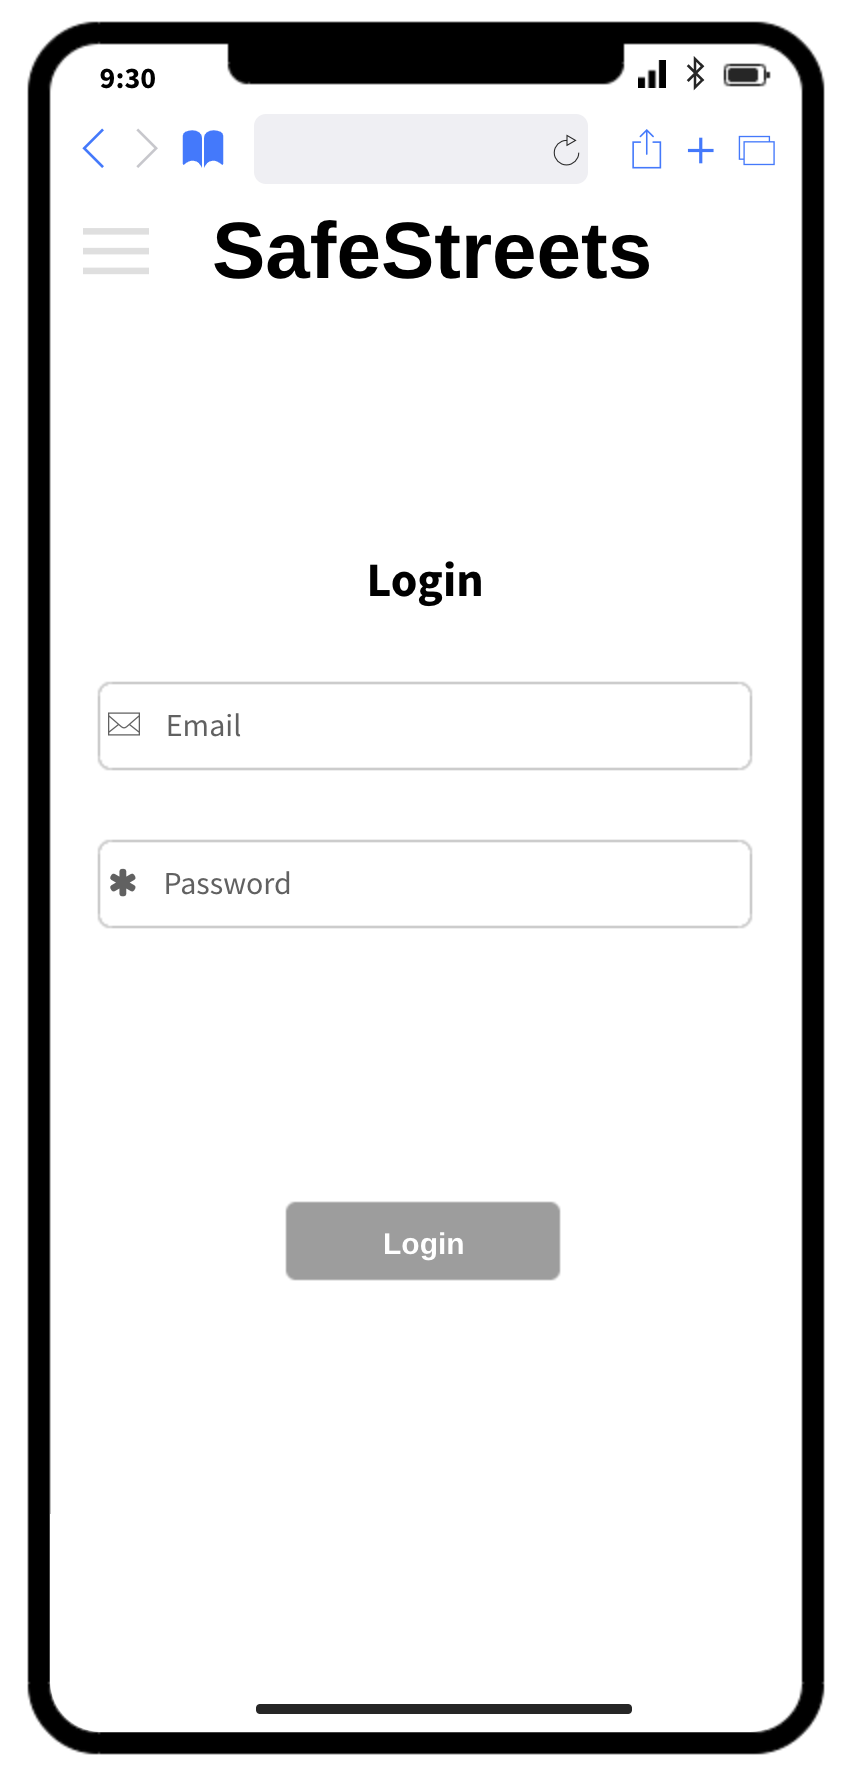
\includegraphics[width=\textwidth]{Images/rasd-mocks/login.png}
			\caption{Login form}
		\end{minipage}
		\hfill
		\begin{minipage}[b]{0.40\textwidth}
			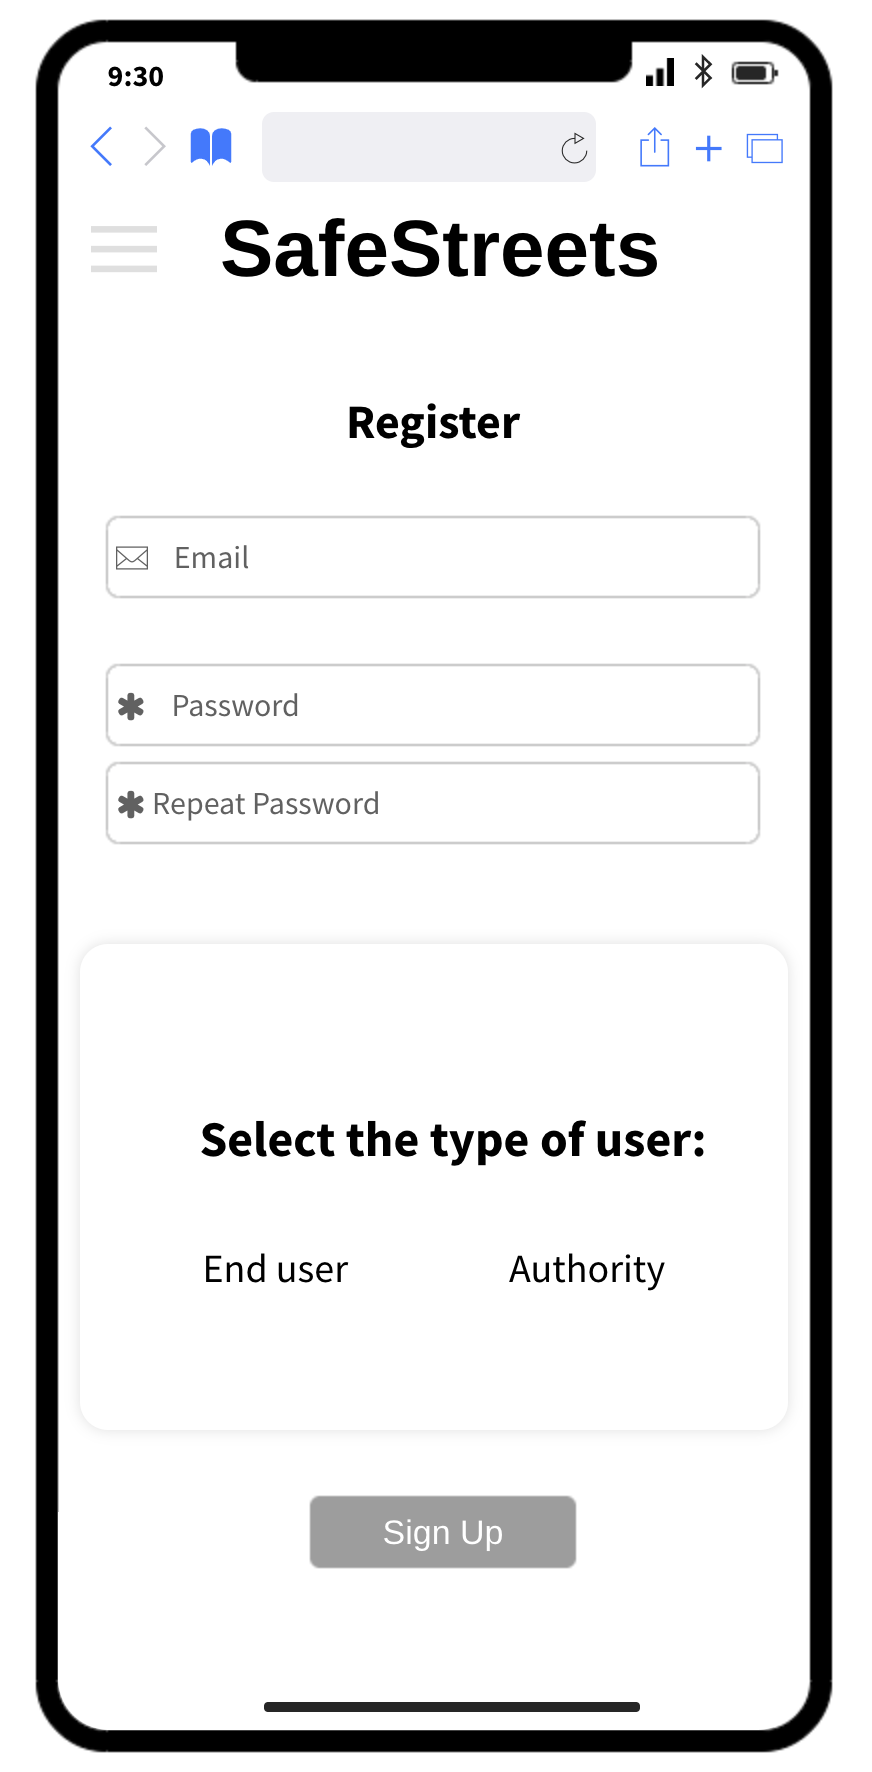
\includegraphics[width=\textwidth]{Images/rasd-mocks/registration.png}
			\caption{Registration form}
		\end{minipage}
	\end{figure}

\newpage
	
		\begin{figure}[H]
		\centering
		\begin{minipage}[b]{0.40\textwidth}
			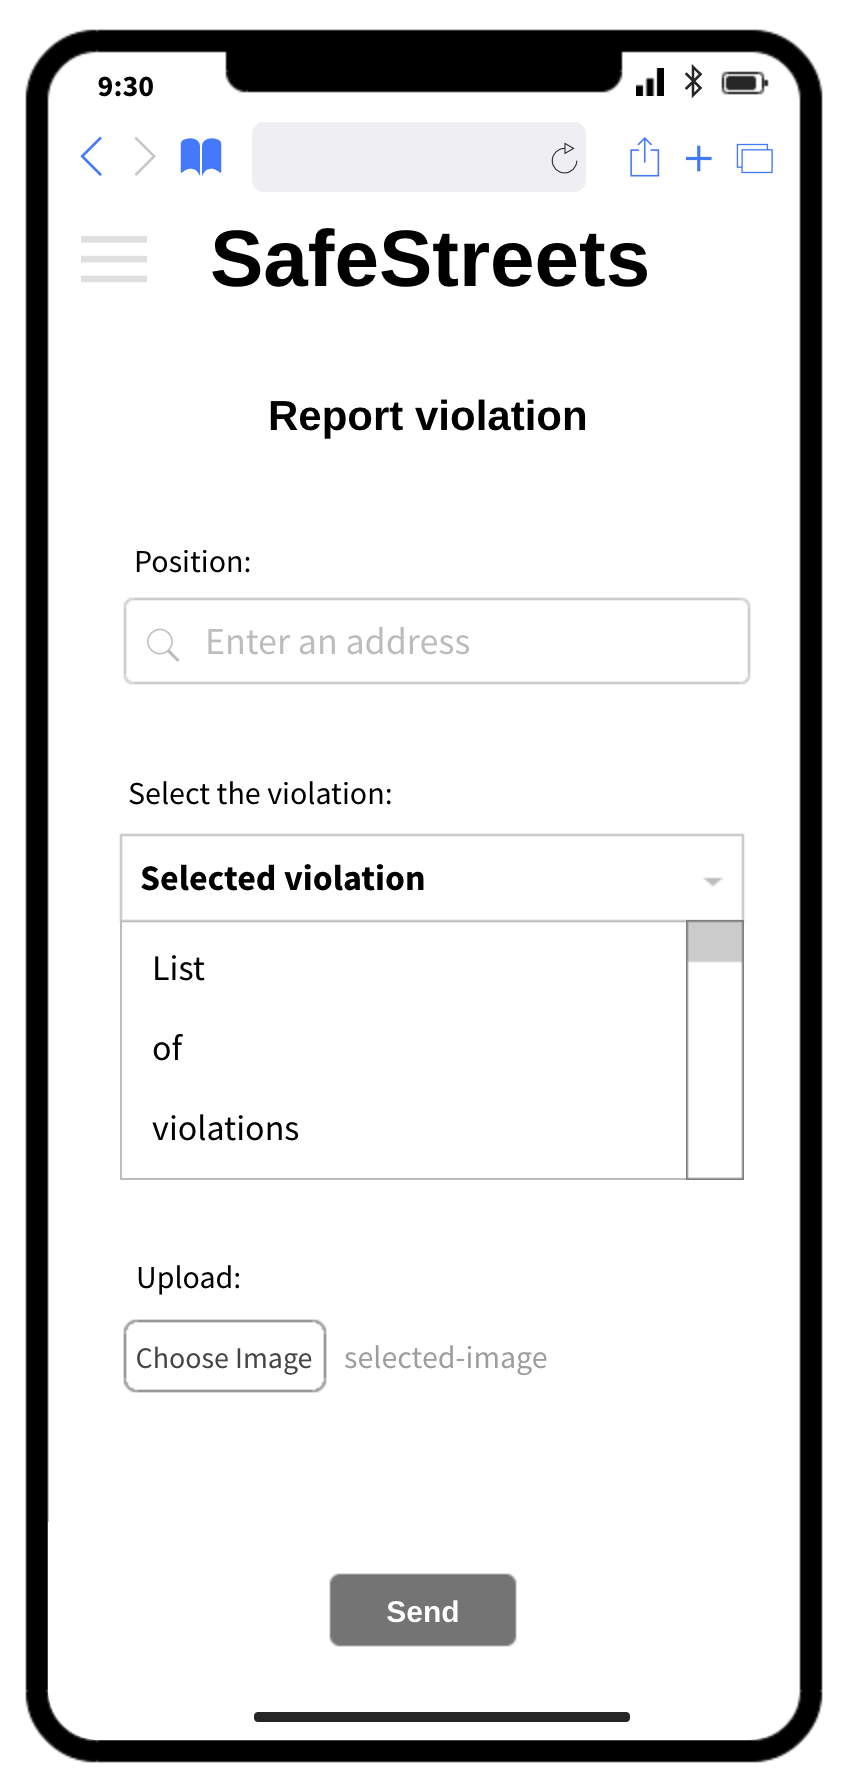
\includegraphics[width=\textwidth]{Images/rasd-mocks/report.png}
			\caption{User send violation report}
		\end{minipage}
		\hfill
		\begin{minipage}[b]{0.40\textwidth}
			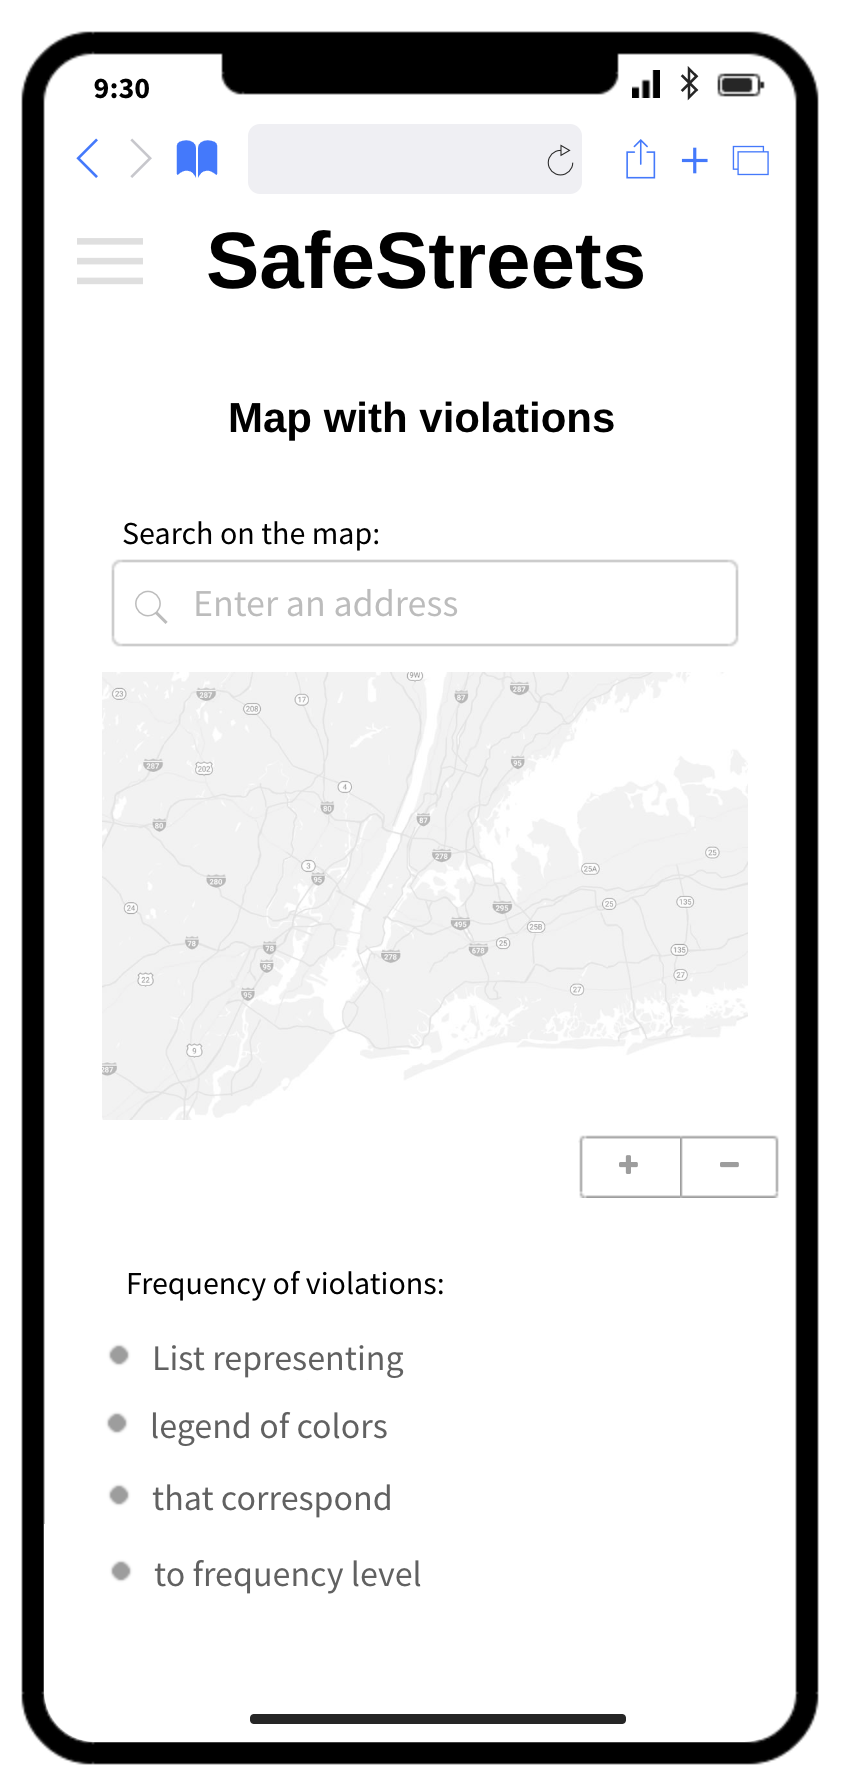
\includegraphics[width=\textwidth]{Images/rasd-mocks/violationsMap.png}
			\caption{Map showing violations}
		\end{minipage}
	\end{figure}

	\begin{figure}[H]
	\centering
	\begin{minipage}[b]{0.40\textwidth}
		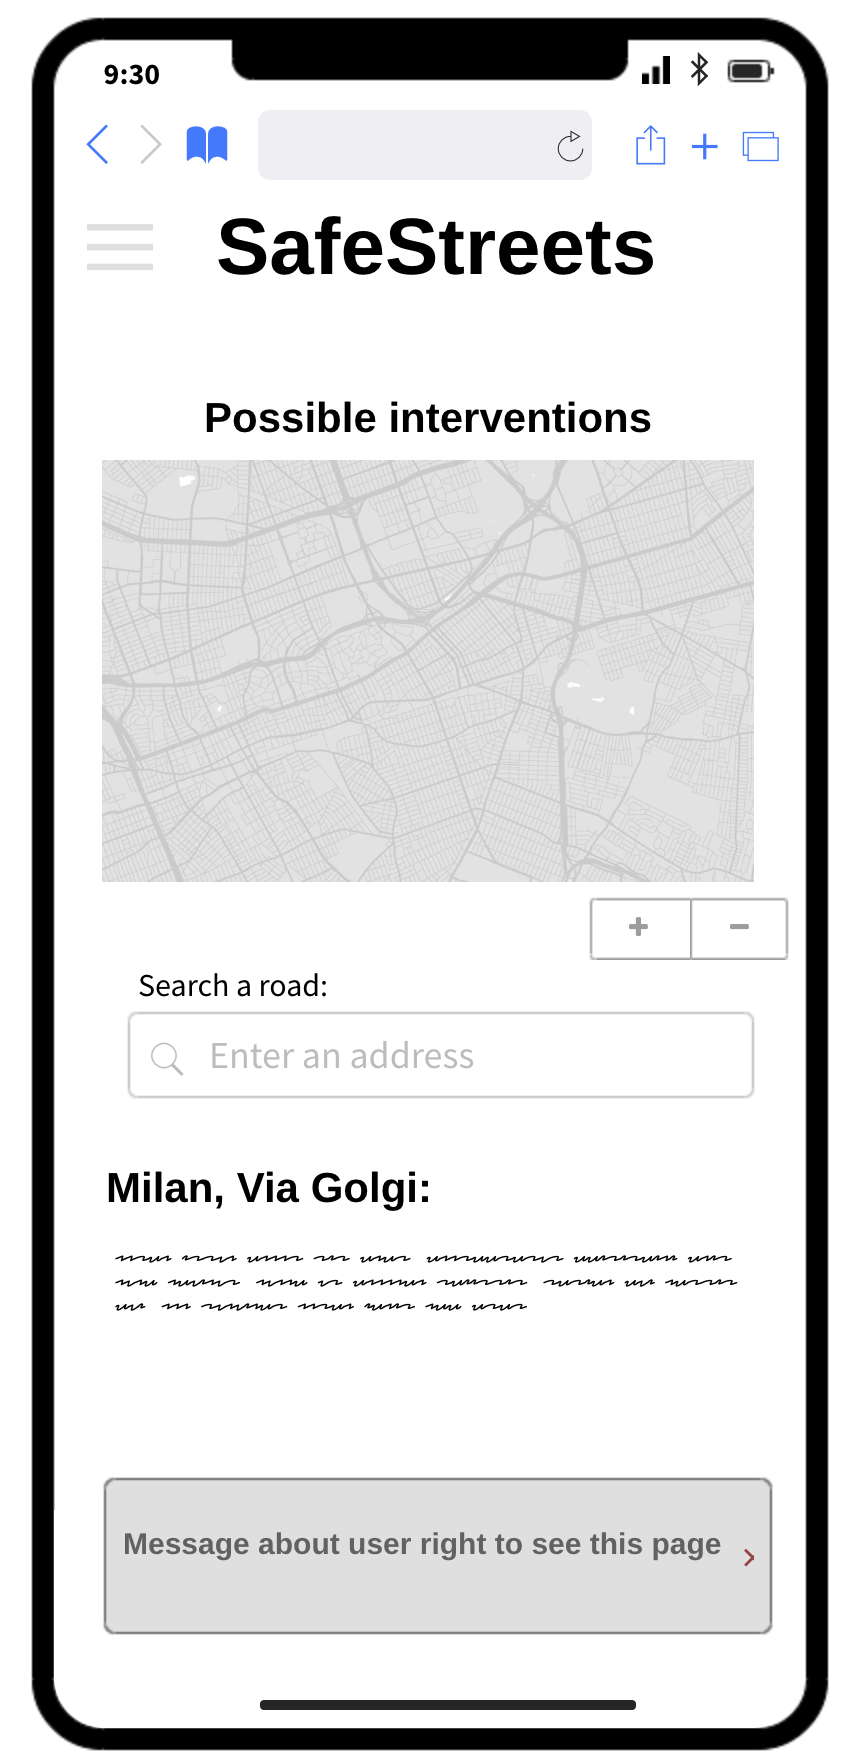
\includegraphics[width=\textwidth]{Images/rasd-mocks/interventions.png}
		\caption{Suggestion for possible interventions}
	\end{minipage}
	\hfill
	\begin{minipage}[b]{0.40\textwidth}
		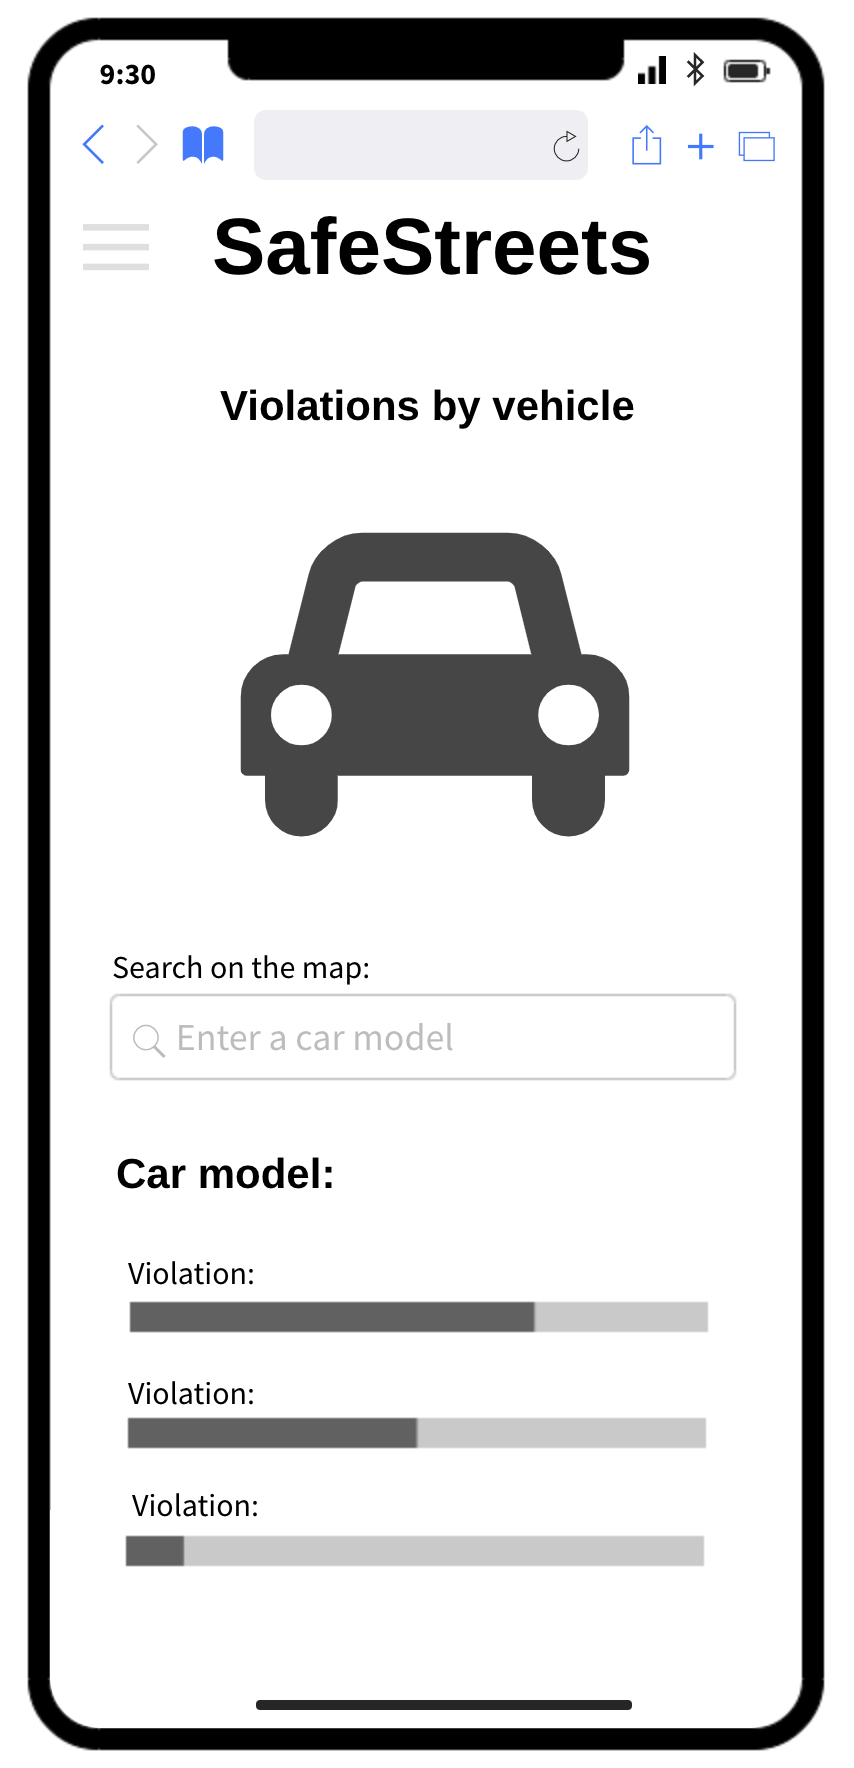
\includegraphics[width=\textwidth]{Images/rasd-mocks/vehicle.png}
		\caption{Violations by vehicle}
	\end{minipage}
\end{figure}

\subsubsection{Hardware interfaces}

\subsubsection{Software interfaces}
The system functionalities are provided without using third part application except for the CUU (Codice Univoco Ufficio) verification. This functions is made by an external web service provided by IndicePA. The code is required during the authorities registration to ensure their identity.
The external API are exposed only for authorities application and the implentation details will be shown in the design document.

\subsubsection{Communication interfaces}
Any communication functionality takes place via internet with HTTP protocol.
More in details, the protocol used is HTTPS, to allow protection and privacy.
This protocol will be used for both access to the web-application and REST communication.

\subsection{Design constraints}
\subsubsection{Standards compliance}
Part of the information collected by Safestreet (ex: license plate) are sensitive. For this reason the project is subject to the General Data Protection Regulation (GDPR). One of the technique used by the system to protect these important information is the creation of different type of user. For example normal account can only send information while authorities have a different account that is able to access to the data colleceted and generated.

\subsubsection{Hardware limitations}
The application is based on retrieving data from the photos sent by the user. Obviously the camera of the devices is a crucial aspect to consider during the design process. For this reason a minimun resolution of the sensor is required to install the application.The identification of this value will be done during design phase and will be written in the design document.
An other constraint is generated by the precision of the gps sensor of the device. Since the impact is smaller than the image resolution, the requirement is not so strict. 

\subsubsection{Any other constraint}
Safestreet works with violations and traffic tickets so it has to deal with law and regulation implications.
For this aspect see the specific domain assumption. 
Furthermore we have to consider the possible improper use of the platform. To prevent it Safestreet do some specific control on the images and is able to detect editing or repeated photos of the same violations. The implementation of this part will be done with some external algorithm and will be detailed in the design document.

\subsection{Functional requirements}
\subsubsection{Definition of use case diagram}
The use case diagrams provide a vision of the uses that can be done with the platform. They show the relationship between the actors and the use that every actor made with the software to reach the goals.

\subsubsection{Scenario 1}
Paul wants to sign up to SafeStreet platform. He has to insert his personal data (name, surname,place,mail etc.) and optionally also the car license plate. He will recieve a confirm mail and can use the platform.
\subsubsection{Scenario 2}
Bob is coming back to his car when he notice that someone has parked in double row and he can’t move. He log in into the safestreet app and he take a picture of the car to report it to the platform which analize the reporting and, in case it is true,it  could generate a traffic ticket and store the data to generate statistics.

\subsubsection{Scenario 3}
Luke is walking on the sidewalk when he see that a young guy is parking on a park reserved for disable.
Luke take a picture of the car and report it to the safestreet platform which analize the reporting and in case it could generate a traffic ticket and store the data to generate statistics.

\subsubsection{Scenario 4}
Mark has submitted a report to the safestreet platform, and he want to check if it has been accepted or declined.
He logs in into the app, he accesses to his reserved area and next to his report there is the status of message sent.

\subsubsection{Scenario 5}
Bill wants to check if someone has made a report on his car. He logs in into the platform and get the access to his profile where he can check if there is any traffic ticket for his car.

\subsubsection{Scenario 6}
The local authority wants to check which are the streets with more reports. They log in into the platform and access to their personal area where they can check the street status. They can set the color of the street based on the reports they recieve but also the platform automatically change the color of the streets based on the reports that recieve through the app.

 
\subsubsection{Scenario 7}
The local authority wants to check which are the vehicle with more reports. They log in into the platform and access to their personal area where they can check the cars that have the most reports assigned. They can set the color of the cars based on the reports they recieve but also the platform automatically change the color of the cars based on the reports that recieve through the app.

\subsubsection{Scenario 8}
The system recieves the photos from the users and have to check if they are true or fake. It runs an alghoritm that can detect if the photo is real or it has been modified. In the first case, the report will be stored and can be generate a traffic ticket. In the second case the report will be discarded.

\subsubsection{Scenario 9}
The local authority have to relase a traffic ticket in case of a user made an infringement. The platform auto-generate the trafic tickets when a report result real, and the local authority recieve a notify.

\subsection{Description of use case scenarios}
\subsubsection{Description scenario 1}


\begin{center}
	\begin{tabular}{ | l | p{6cm} | } 
		\hline
		ACTORS & Visitors  \\ 
		\hline
		GOALS & Sign up  \\ 
		\hline
		INPUT CONDITION & Personal data (name, surname, mail, telephone number, place where he lives, car license plate etc.)  \\ 
		\hline
		EVENTS FLOW & The user from the home page clicks on sign up. He inserts all of his information and if it is all correct he will recive an email of confirm.  \\ 
		\hline
		OUTPUT CONDITION & The user can now log in and use all the function that the user can do on the platform.  \\ 
		\hline
		EXCEPTIONS & Data incorrect, user already exists, mail already exists. All of this exceptions will be notified instantly to the user. \\ 
		\hline
	\end{tabular}
\end{center}

\subsubsection{Description scenario 2}

\begin{center}
	\begin{tabular}{ | l | p{6cm} | } 
		\hline
		ACTORS & User  \\ 
		\hline
		GOALS & Report a violation  \\ 
		\hline
		INPUT CONDITION & Type of violation (double row park), name of the street,  \\ 
		\hline
		EVENTS FLOW & The user take a picture of the car that has done the violation. The system use an algorithm to read the car license plate and then store all the informations once it is established that the photo isn't fake.  \\ 
		\hline
		OUTPUT CONDITION & The violation has been stored with all the data, it will be generated a traffic ticket, and the local authority can decide to highlight who has made the violation or the street. \\ 
		\hline
		EXCEPTIONS & Data incorrect or fake photo. The report will be discarded and no traffic ticket will be generated.  \\ 
		\hline
	\end{tabular}
\end{center}

\subsubsection{Description scenario 3}

\begin{center}
	\begin{tabular}{ | l | p{6cm} | } 
		\hline
		ACTORS & User  \\ 
		\hline
		GOALS & Report a violation  \\ 
		\hline
		INPUT CONDITION & Type of violation (wrong park), name of the street,  \\ 
		\hline
		EVENTS FLOW & The user take a picture of the car that has done the violation. The system use an algorithm to read the car license plate and then store all the informations once it is established that the photo isn't fake.  \\ 
		\hline
		OUTPUT CONDITION & The violation has been stored with all the data, it will be generated a traffic ticket, and the local authority can decide to highlight who has made the violation or the street. \\ 
		\hline
		EXCEPTIONS & Data incorrect or fake photo. The report will be discarded and no traffic ticket will be generated.  \\ 
		\hline
	\end{tabular}
\end{center}

\subsubsection{Description scenario 4}

\begin{center}
	\begin{tabular}{ | l | p{6cm} | } 
		\hline
		ACTORS & User  \\ 
		\hline
		GOALS & Check report status  \\ 
		\hline
		INPUT CONDITION & User credentials  \\ 
		\hline
		EVENTS FLOW & The user log in into the platform. He accesses to his personal area and he can check the status of his report \\ 
		\hline
		OUTPUT CONDITION & Report status \\ 
		\hline
		EXCEPTIONS & The user hasn't made any report. The system show a messagge that the list of the reports is empty.  \\ 
		\hline
	\end{tabular}
\end{center}

\subsubsection{Description scenario 5}

\begin{center}
	\begin{tabular}{ | l | p{6cm} | } 
		\hline
		ACTORS & User  \\ 
		\hline
		GOALS & Check his profile  \\ 
		\hline
		INPUT CONDITION & User credentials  \\ 
		\hline
		EVENTS FLOW & The user log in into the platform. He accesses to his personal area and he can check if his car has recieved some report \\ 
		\hline
		OUTPUT CONDITION & Car status \\ 
		\hline
		EXCEPTIONS & The user hasn't a car or hasn't recived any report. The system show a messagge that there isn't any report.  \\ 
		\hline
	\end{tabular}
\end{center}

\subsubsection{Description scenario 6}

\begin{center}
	\begin{tabular}{ | l | p{6cm} | } 
		\hline
		ACTORS & Local authority  \\ 
		\hline
		GOALS & Check streets status  \\ 
		\hline
		INPUT CONDITION & Local authority credentials  \\ 
		\hline
		EVENTS FLOW & The authority log in into the platform. He accesses to his personal area and he can check the streets status \\ 
		\hline
		OUTPUT CONDITION & Different colors for the streets based on their status and possibly changes to the color of some streets \\ 
		\hline
		EXCEPTIONS & none \\ 
		\hline
	\end{tabular}
\end{center}

\subsubsection{Description scenario 7}

\begin{center}
	\begin{tabular}{ | l | p{6cm} | } 
		\hline
		ACTORS & Local authority  \\ 
		\hline
		GOALS & Check cars status  \\ 
		\hline
		INPUT CONDITION & Local authority credentials  \\ 
		\hline
		EVENTS FLOW & The authority log in into the platform. He accesses to his personal area and he can check the cars status based on reports \\ 
		\hline
		OUTPUT CONDITION & Different colors for the cars based on how many reports they recived and possibly changes to the color of some cars \\ 
		\hline
		EXCEPTIONS & none \\ 
		\hline
	\end{tabular}
\end{center}

\subsubsection{Description scenario 8}

\begin{center}
	\begin{tabular}{ | l | p{6cm} | } 
		\hline
		ACTORS & SafeStreets  \\ 
		\hline
		GOALS & Check the reliability of the photo  \\ 
		\hline
		INPUT CONDITION & Photo that has been taken by a user.  \\ 
		\hline
		EVENTS FLOW & The system recives from the user a photo of a possibile violation. It runs an algorithm that can establish if it is real or fake. \\ 
		\hline
		OUTPUT CONDITION & The photo is real of fake. \\ 
		\hline
		EXCEPTIONS & none \\ 
		\hline
	\end{tabular}
\end{center}

\subsubsection{Description scenario 9}

\begin{center}
	\begin{tabular}{ | l | p{6cm} | } 
		\hline
		ACTORS & SafeStreets  \\ 
		\hline
		GOALS & Generate trafic tickets  \\ 
		\hline
		INPUT CONDITION & Report  \\ 
		\hline
		EVENTS FLOW & If the report is real than it could be generated the trafic ticket based on the type of violation the user has committed. \\ 
		\hline
		OUTPUT CONDITION & Trafic ticket \\ 
		\hline
		EXCEPTIONS & The report is fake, nothing is generated. \\ 
		\hline
	\end{tabular}
\end{center}
\newpage
\subsection{Sequence diagram}
\subsubsection{Scenario 2}
	\begin{figure}[H]
	\begin{minipage}[b]{0.40\textwidth}
		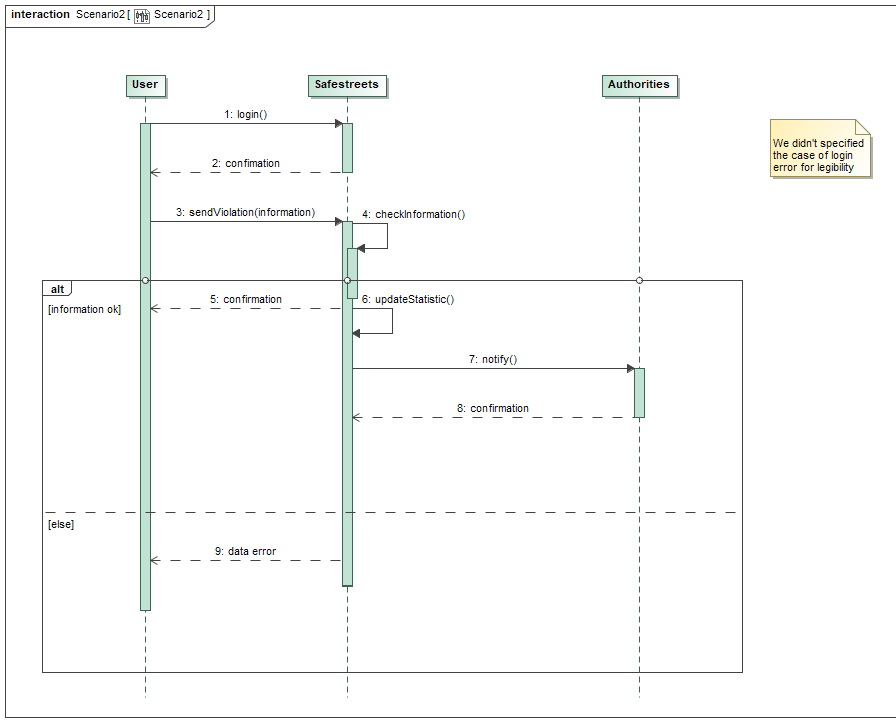
\includegraphics[width=18cm,height=15cm]{Images/SequenceRASD/Scenario2.png}
		\caption{Scenario 2}
	\end{minipage}
\end{figure}
\subsubsection{Scenario 5}
\begin{figure}[H]
	\begin{minipage}[b]{0.40\textwidth}
		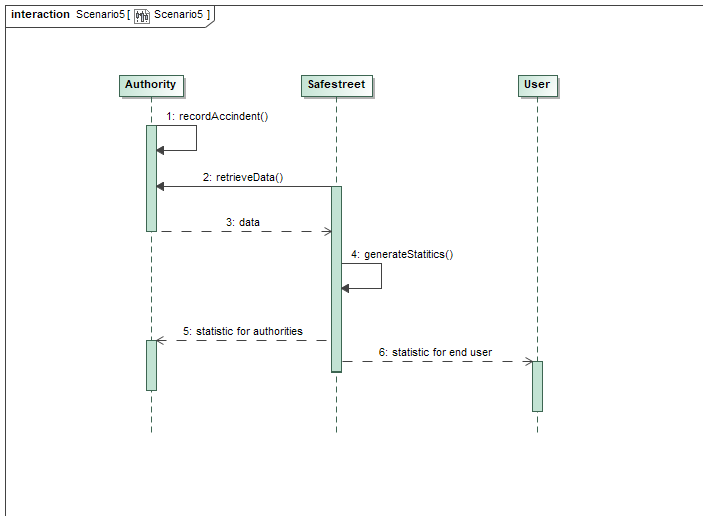
\includegraphics[width=15cm,height=10cm]{Images/SequenceRASD/Scenario5.png}
		\caption{Scenario 5}
	\end{minipage}
\end{figure}
\subsubsection{Scenario 6}
\begin{figure}[H]
	\begin{minipage}[b]{0.40\textwidth}
		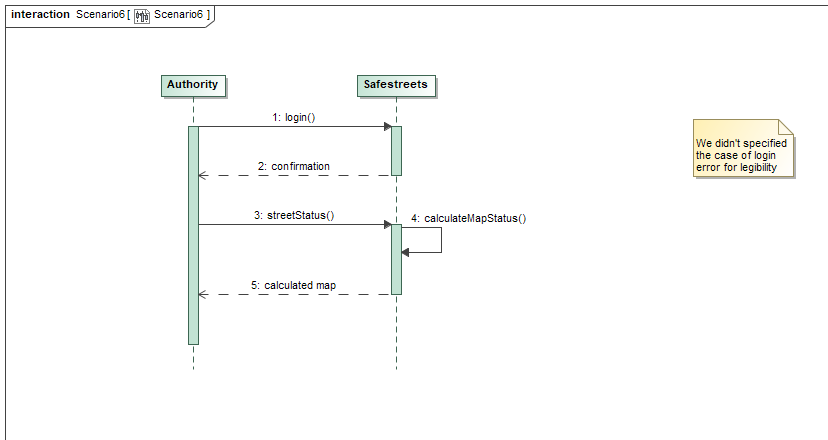
\includegraphics[width=15cm,height=10cm]{Images/SequenceRASD/Scenario6.png}
		\caption{Scenario 6}
	\end{minipage}
\end{figure}

\subsection{Software system attributes}
\subsubsection{Reliability}
The system has to ensure reliability, to this scope we have decided to keep a backup server, that operate every 24h.
The system also use an algorithm to ensure that the reports of violations that the system recive, are real and not modified or fake.
\subsubsection{Availability}
The platform has to be available every day, especially in the rush hours because are the hours where there are more traffic and it could be useful to be active in that time. SafeStreets must have 99\% (3.65 days/year downtime).
\subsubsection{Security}
The data have to be crypted, to grant the privacy (ex.user's position, car license plate etc.). It could be useful to use HTTPS protocol to transmit data from user to SafeStreets.
Every account must have a strong password with the combination of upper-case, lower-case letters, numbers and punctuation.
\subsubsection{Maintainability}
The system is programmed to be compatible with other platform, like the system of the local authority.
There could be maintenance interventions, when it's possible there will be in the hours with the less use of the platform.
There will be released updates, both for application and system.
\subsubsection{Portability}
The entire system is portable, every user (citizen or local authority) can access to their profile, see data, statisthics and make reports of violation from their mobile or their tablet, not especially from PCs.
\subsection{Mapping on requirements}
\begin{center}
	\begin{tabular}{ | l | p{2cm} | p{2cm}| p{2cm}|} 
		\hline
		 RawID & GoalID & ReqID & Use Case ID \\
		\hline
		1&G1&RE.1&Scenario 2/3\\
		\hline
		2&G2.1&RE.2&\\
		\hline
		3&G2&RE.3&\\
		\hline
		4&G3.1&RE.4&Scenario 6\\
		\hline
		5&G3&RE.5&\\
		\hline
		6&G4&RE.6&\\
		\hline
		7&G5&RE.7&Scenario 8\\
		\hline
		8&G2&RE.8&Scenario 9\\
		\hline
	\end{tabular}
\end{center}


 